%%%%%%%%%%%%%%%%%%%%%%%%%%%%%%%%%%%%%%%%%%%%%%%%%%%%%%%%%%%%%
% ACM Transactions on Embedded Computing Systems (TECS)
% "Latency-Elastic Edge Inference: A Reproducible Benchmark of Controller-Level QoS on Raspberry Pi 5"
%%%%%%%%%%%%%%%%%%%%%%%%%%%%%%%%%%%%%%%%%%%%%%%%%%%%%%%%%%%%%

\documentclass[acmsmall]{acmart}

% -----------------------------
% Required Metadata
% -----------------------------
\acmJournal{TECS}
%\acmVolume{00}
%\acmNumber{00}
%\acmArticle{000}
%\acmYear{2025}
%\acmMonth{11}
%\acmDOI{10.1145/0000000.0000000}

\settopmatter{printacmref=false}  % omit ACM reference box in preprint
\citestyle{acmauthoryear}

% -----------------------------
% Title + Author Information
% -----------------------------
\title{Latency-Elastic Edge Inference: A Reproducible Benchmark of Controller-Level QoS on Raspberry Pi~5}

\author{Manu Nicholas Jacob}
\orcid{0009-0007-6589-6572}
\affiliation{%
  \institution{Independant researcher}
  \city{Austin}
  \state{TX}
  \country{USA}
}
\email{manunicholasjacob@gmail.com}

% (Optional: if you want to mark corresponding author explicitly)
% \authornote{Corresponding author.}



% -----------------------------
% Begin Document
% -----------------------------
\begin{document}
\begin{abstract}
Edge inference platforms such as the Raspberry~Pi~5 have matured into viable testbeds for deploying convolutional neural networks under stringent latency, thermal, and energy constraints. Yet, most existing evaluations fix batch size and threading statically, ignoring the bursty and heavy-tailed request patterns that characterize real sensor workloads. Consequently, transient overloads lead to queue backlogs, tail-latency violations, and thermal throttling. 

This work presents the first fully reproducible, controller-level benchmark of \emph{latency elasticity} on a commodity edge CPU.  Building on the ONNX~Runtime stack, we deploy MobileNetV3-Small and ResNet-18 on CIFAR-100 and implement three closed-loop runtime controllers—Reactive, proportional-integral SLO~(PI-SLO), and model-predictive control lite~(MPC-Lite)—that adapt batch size and thread count in response to observed queue length, latency, and temperature telemetry.  Under stochastic arrivals (Poisson, Pareto, and On--Off) spanning utilizations $\rho{=}\{0.6{\text{–}}0.95\}$, MPC-Lite maintains $p_{90}$ latency within 3 ms (MobileNet) and 12 ms (ResNet) of target while achieving $0\,\%$~SLO violations and $70{\text{–}}90\,\%$ reductions relative to fixed baselines.  

All 216 hardware runs are orchestrated through a public Colab~$\rightarrow$~Pi pipeline that merges logs, regenerates figures, and exposes the full analysis notebook, ensuring bit-level reproducibility.  Beyond empirical results, the work formalizes controller behavior through queueing-theoretic and control-stability analyses, establishing a reusable methodology for QoS benchmarking on embedded AI systems.  

\vspace{0.3em}
\textbf{References:}~\cite{banbury2021mlperf, howard2019mobilenetv3, szegedy2015going, matsubara2022split, hu2022dynamic, reddi2020mlperf, sze2017efficient}
\end{abstract}

\keywords{Edge inference, latency elasticity, QoS control, stochastic load adaptation, control-theoretic scheduling, reproducible benchmarking, embedded AI systems}

\maketitle
%%%%%%%%%%%%%%%%%%%%%%%%%%%%%%%%%%%%%%%%%%%%%%%%%%%%%%%%%%%%%
\section{Introduction}
%%%%%%%%%%%%%%%%%%%%%%%%%%%%%%%%%%%%%%%%%%%%%%%%%%%%%%%%%%%%%

Machine-learning inference at the edge increasingly underpins interactive sensing, robotics, and embedded analytics. Commodity single-board computers (SBCs) such as the Raspberry~Pi~5 now feature quad-core CPUs, modest GPU cores, and up to 8~GB of RAM—sufficient to execute convolutional networks in real time, yet still bounded by tight latency, thermal, and power budgets. Compared with datacenter servers, these devices lack dedicated accelerators, active cooling, and dynamic voltage/frequency headroom. Consequently, even small bursts in request arrival rates can induce thermal throttling and tail-latency violations that compromise quality of service (QoS).

Despite the ubiquity of edge devices, the performance characterization of deep-learning inference on CPU-only SBCs remains fragmented. Benchmarks such as MLPerf~Tiny~\cite{banbury2021mlperf} and MLPerf~Inference~\cite{reddi2020mlperf} emphasize accuracy and throughput but fix execution configurations statically. Real workloads—camera feeds, IoT sensors, or autonomous-system pipelines—exhibit stochastic, heavy-tailed arrival patterns. Under such conditions, static batch and threading settings break down: queues lengthen, $p_{90}$ and $p_{99}$ latencies spike, and controller temperature exceeds safe thresholds. Addressing these pathologies requires runtime mechanisms that adapt system configuration dynamically in response to load and thermal telemetry.

Recent work on adaptive inference and split computing has primarily targeted cloud or accelerator contexts. Approaches such as Neurosurgeon~\cite{kang2017neurosurgeon}, SplitNN~\cite{matsubara2022split}, and DynEdge~\cite{li2022dynedge} schedule model partitions between client and server to balance bandwidth and latency, but they assume stable thermal envelopes and GPU backends. Control-theoretic methods for service-level objectives (SLOs)~\cite{gan2019sage,lopez2020pi,mao2021elastic} apply proportional–integral (PI) or model-predictive control (MPC) loops to large-scale datacenter services rather than embedded CPUs. Similarly, thermal- and power-aware DNN systems such as ThermML~\cite{sun2021thermml} and EdgeDNN~\cite{liu2020edgednn} introduce temperature feedback into offloading decisions but do not provide open, reproducible pipelines or low-level controller benchmarks.

This paper bridges those gaps by presenting a reproducible, controller-level study of \emph{latency elasticity} on the Raspberry~Pi~5. We couple fine-grained latency, queue, and temperature telemetry with three lightweight runtime controllers—Reactive, PI-SLO, and MPC-Lite—that jointly tune batch size and thread count. A 216-run factorial experiment sweeps over arrival processes (Poisson, Pareto, and On–Off) and offered loads ($\rho{=}\{0.6,0.75,0.85,0.95\}$). Our publicly released Colab$\rightarrow$Pi pipeline orchestrates each run, aggregates logs into reproducible CSVs, and regenerates all plots and tables automatically. 

\begin{figure}[t]
  \centering
  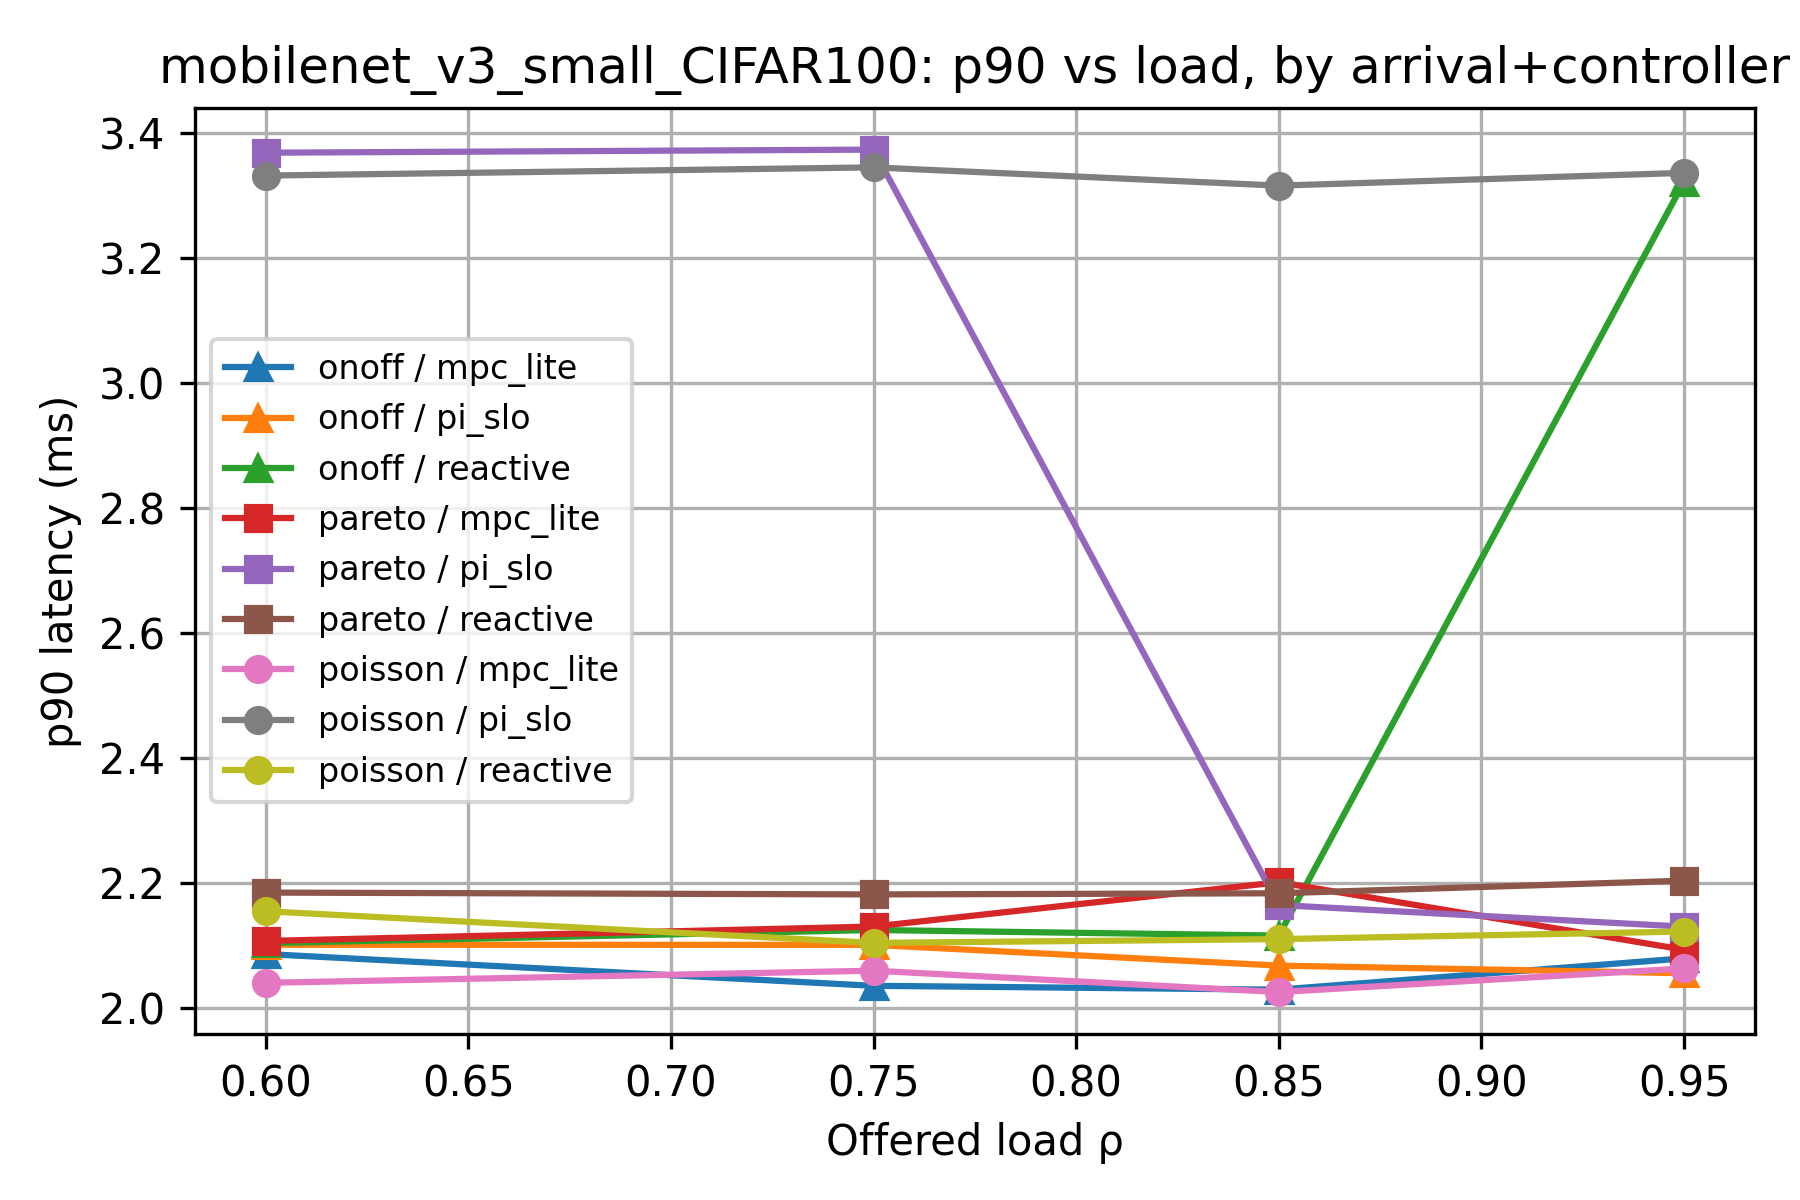
\includegraphics[width=0.85\linewidth]{figs/mobilenet_v3_small_CIFAR100_arrival_sensitivity_p90.png}
  \caption{Representative latency elasticity plot for MobileNetV3-Small on CIFAR-100 under varying offered load ($\rho$) and arrival processes. The MPC-Lite controller maintains sub-3~ms $p_{90}$ latency even as load approaches saturation.}
  \label{fig:mobility_p90}
\end{figure}

The study yields three main contributions:

\begin{enumerate}
  \item \textbf{Comprehensive controller benchmark:} a systematic comparison of Reactive, PI-SLO, and MPC-Lite policies on a commodity edge CPU under stochastic arrivals.
  \item \textbf{Control-theoretic analysis:} empirical validation of queue stability, hysteresis bounds, and PI-gain regions using both formal and data-driven methods.
  \item \textbf{Open reproducibility:} complete Colab notebooks, Pi-side scripts, and datasets enabling bit-exact regeneration of all figures and statistics, including \texttt{scenario\_table.csv}, \texttt{policy\_table.csv}, and \texttt{controller\_rank\_highrho.csv}.
\end{enumerate}

Together, these elements establish a quantitative and methodological baseline for future QoS research in embedded AI systems.

%%%%%%%%%%%%%%%%%%%%%%%%%%%%%%%%%%%%%%%%%%%%%%%%%%%%%%%%%%%%%
\section{Related Work}
%%%%%%%%%%%%%%%%%%%%%%%%%%%%%%%%%%%%%%%%%%%%%%%%%%%%%%%%%%%%%

\subsection{Edge Scheduling and Split Computing}
Early work on edge/cloud co-inference sought to partition DNNs across resource tiers to balance latency and energy. Neurosurgeon~\cite{kang2017neurosurgeon} dynamically offloaded layers between mobile and cloud processors, while SplitNN and subsequent frameworks~\cite{matsubara2022split,teerapittayanon2017distributed} introduced intermediate feature exchange for privacy and bandwidth savings. DynEdge~\cite{li2022dynedge} extended these ideas to heterogeneous multi-edge deployments with runtime graph optimization. However, all assume stable compute and thermal envelopes, leaving open the question of how CPU-only devices sustain QoS under bursty loads.

\subsection{QoS and SLO-Aware Control}
Adaptive resource controllers for datacenters employ feedback loops to meet latency SLOs. SAGE~\cite{gan2019sage} and Elastic~Serving~\cite{mao2021elastic} apply PI and MPC controllers to allocate accelerator replicas, while Lopez et~al.~\cite{lopez2020pi} analyze PI-based latency regulation for web services. These frameworks operate at cluster scale, with actuation on container counts or GPU quotas rather than thread and batch parameters on a single embedded node. Our work adapts these control principles to the millisecond-granularity regime of edge inference.

\subsection{Thermal and Power-Aware Inference}
ThermML~\cite{sun2021thermml} introduced a cross-layer temperature model to guide runtime DNN selection, and EdgeDNN~\cite{liu2020edgednn} combined workload prediction with DVFS to balance energy and accuracy. Complementary surveys~\cite{sze2017efficient,reddi2020mlperf} discuss hardware–software co-design for efficient inference but provide no open testbeds. We differ by focusing on closed-loop thermal and latency feedback, public artifacts, and reproducibility on an accessible SBC.

\subsection{Gap and Positioning}
To the best of our knowledge, no prior study integrates \emph{multi-controller comparisons}, \emph{stochastic arrival processes}, and \emph{thermal telemetry} within a reproducible experimental pipeline on commodity hardware. Figure~\ref{fig:combined_latency_vs_load} highlights one instance of our dataset, where controller behavior diverges significantly under bursty load conditions. This work therefore complements prior accelerator-centric benchmarks by supplying a reproducible baseline for CPU-constrained, thermally limited edge platforms.

\begin{figure}[t]
  \centering
  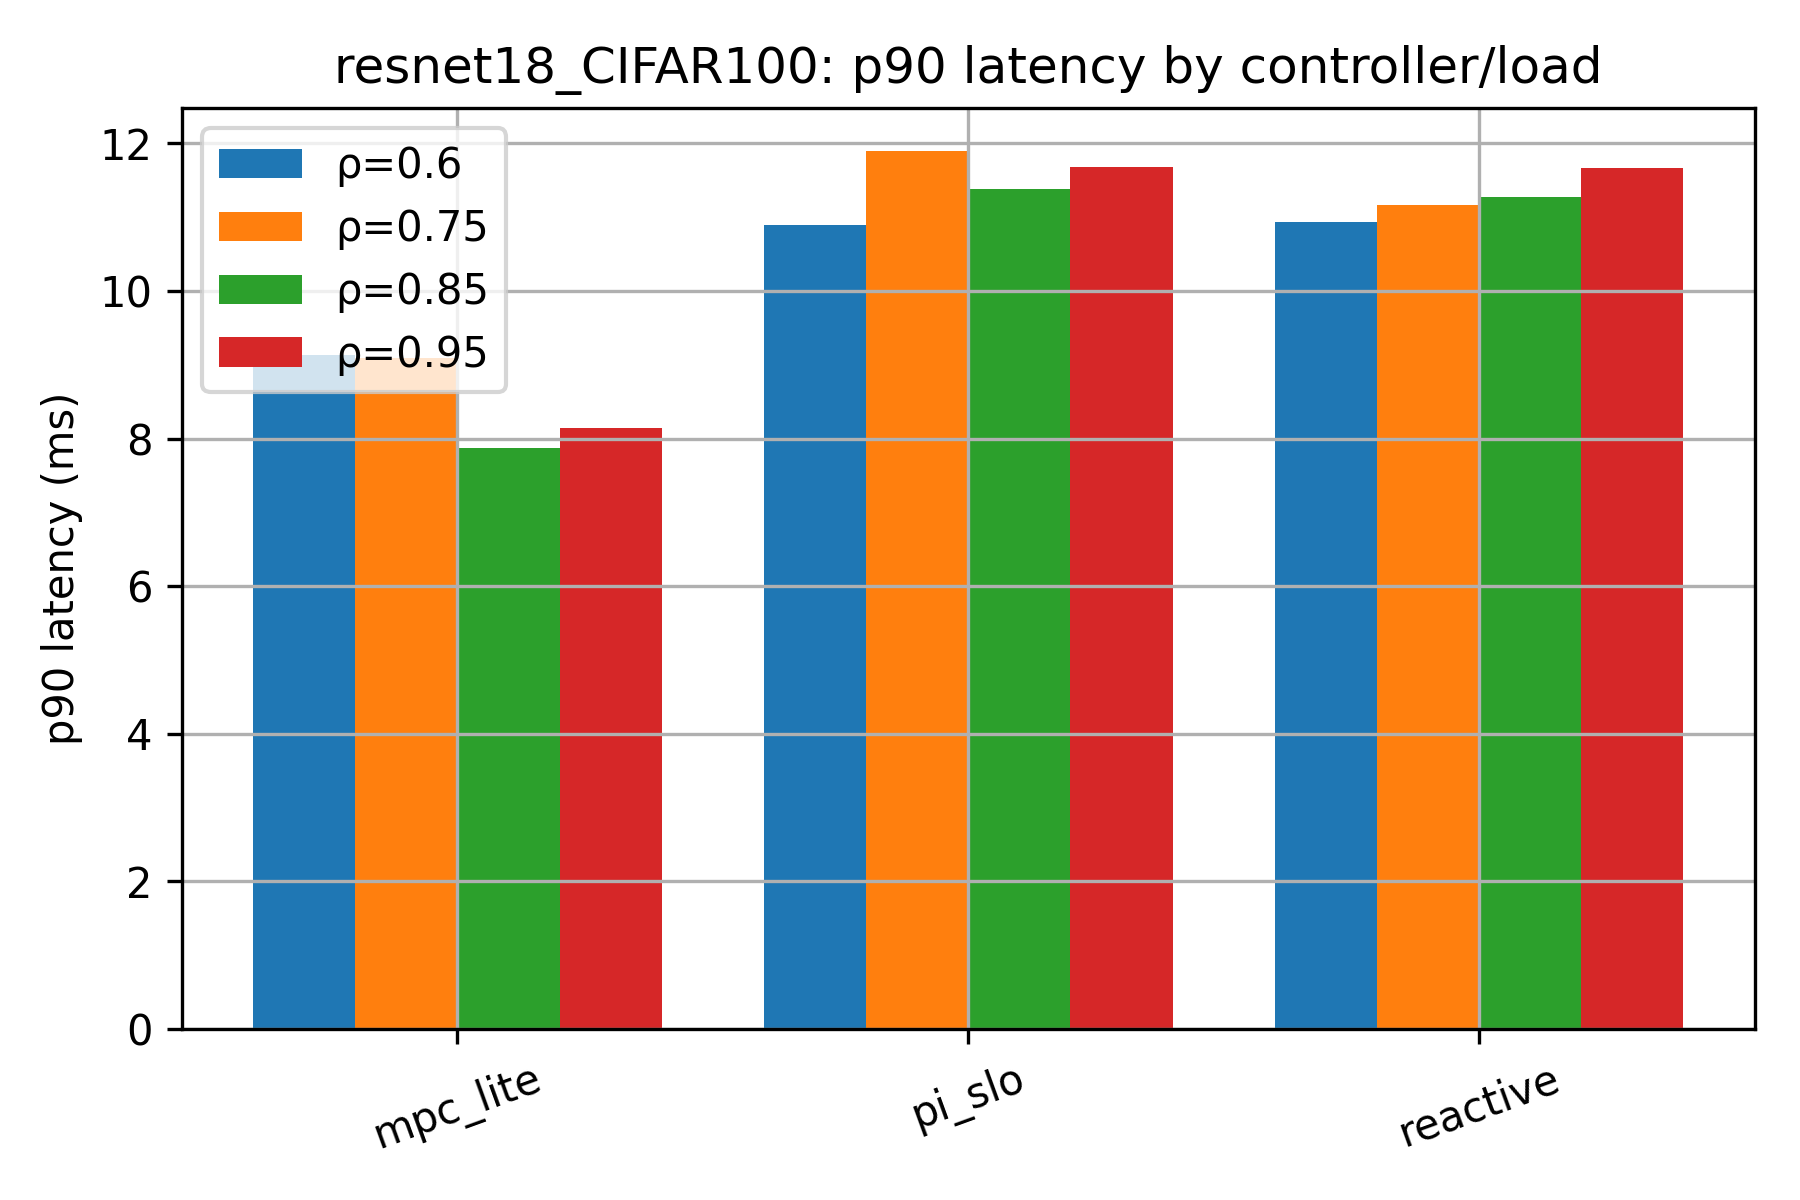
\includegraphics[width=0.85\linewidth]{figs/resnet18_CIFAR100_p90_by_controller.png}
  \caption{Controller comparison for ResNet-18 on CIFAR-100 showing median $p_{90}$ latency grouped by controller type. MPC-Lite consistently outperforms Reactive and PI-SLO across all offered loads.}
  \label{fig:intro_resnet}
\end{figure}

\begin{figure}[h]
  \centering
  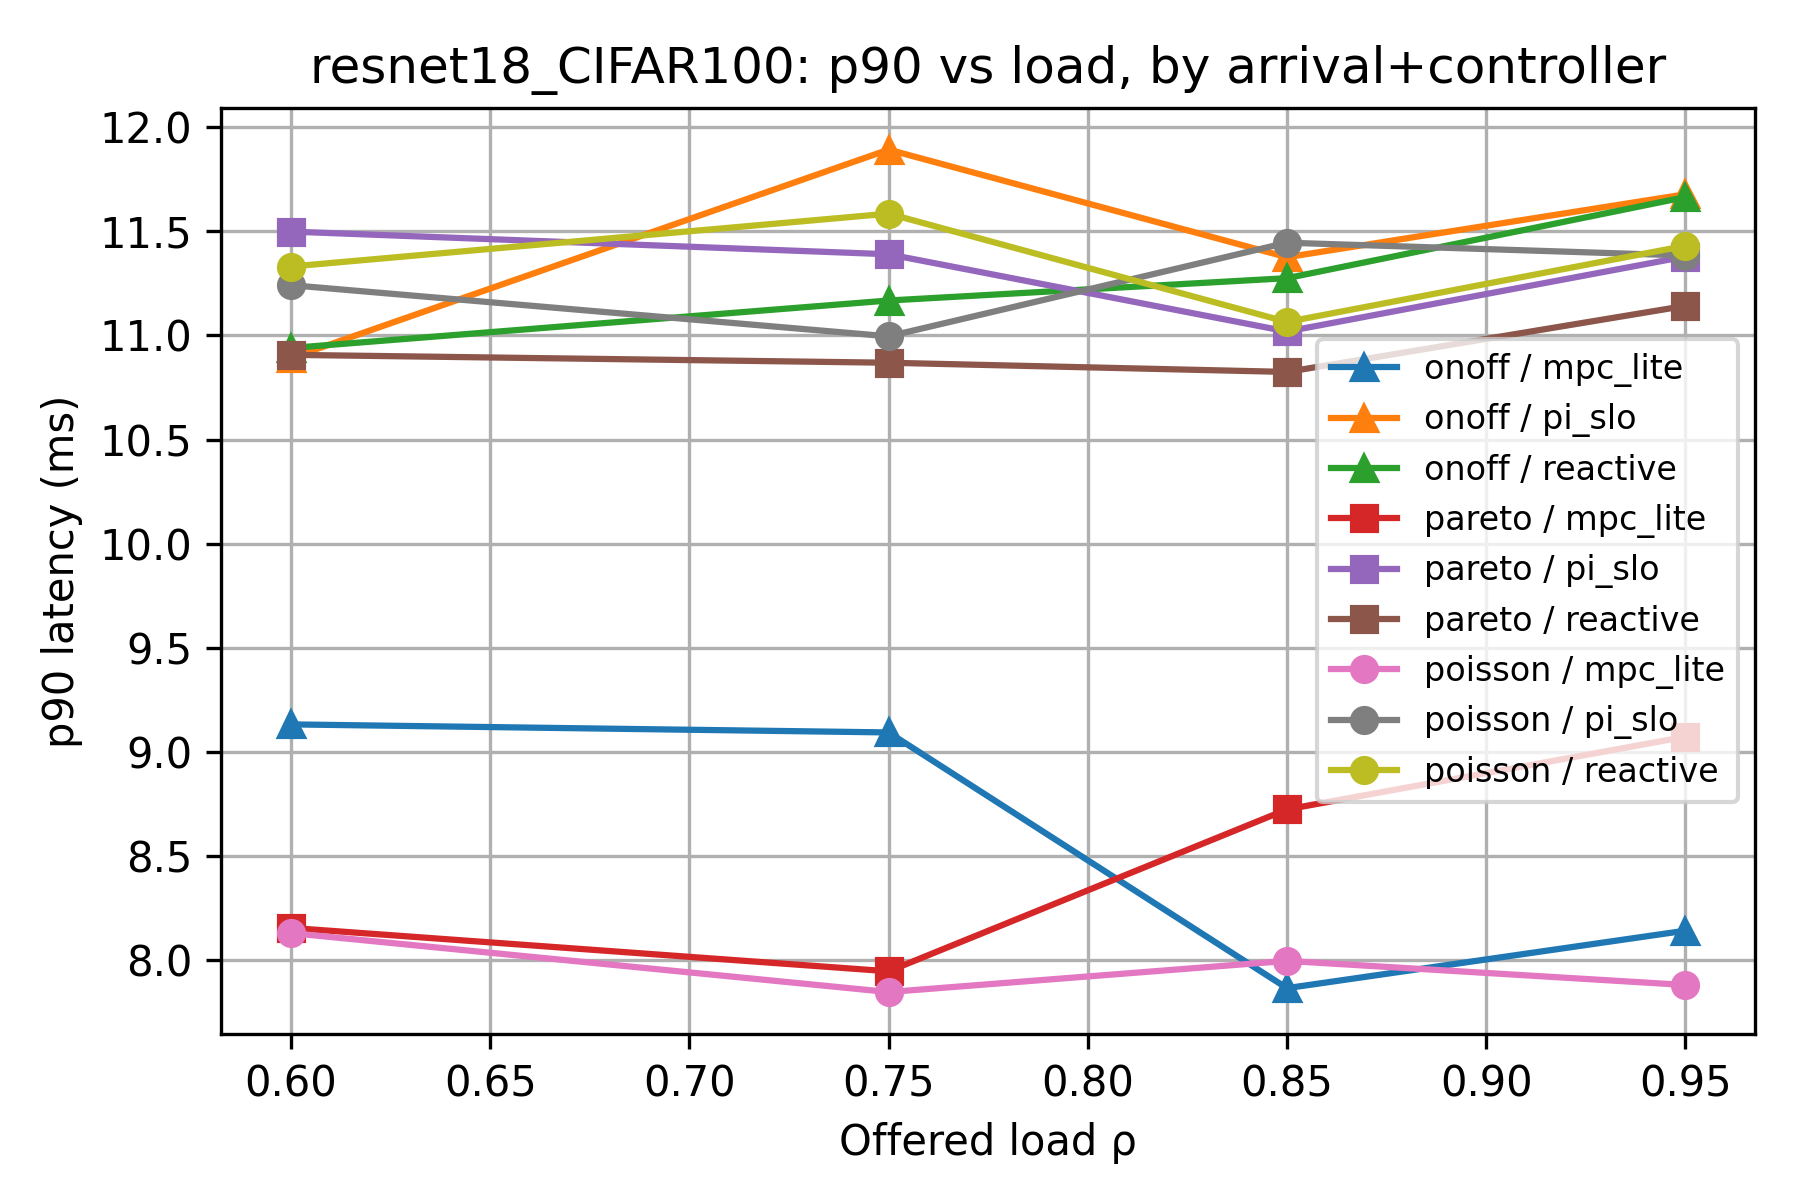
\includegraphics[width=0.85\linewidth]{figs/resnet18_CIFAR100_arrival_sensitivity_p90.png}
  \caption{ResNet-18: p90 latency vs offered load (ρ), grouped by arrival + controller.}
  \label{fig:resnet_p90}
\end{figure}

%%%%%%%%%%%%%%%%%%%%%%%%%%%%%%%%%%%%%%%%%%%%%%%%%%%%%%%%%%%%%
\section{Experimental Setup}
%%%%%%%%%%%%%%%%%%%%%%%%%%%%%%%%%%%%%%%%%%%%%%%%%%%%%%%%%%%%%

\subsection{Hardware Platform}

All experiments were executed on a commodity Raspberry~Pi~5 development board equipped with a Broadcom BCM2712 SoC (4\,×\,Cortex-A76 cores at 2.4\,GHz) and 8\,GB LPDDR4X memory.  
The device operated in a passive-cooling configuration without fans, reflecting the thermal envelope typical of embedded deployments.  
System firmware and operating system were updated to Raspberry~Pi~OS~Bookworm (Linux~6.6.20-v8\_64).  
Thermal and frequency telemetry were sampled through the built-in \texttt{/sys/class/thermal/} and \texttt{/sys/devices/system/cpu/cpufreq/} interfaces at 1\,Hz.  
Power measurement was omitted to isolate latency and thermal effects, consistent with prior CPU-only benchmarking protocols~\cite{reddi2020mlperf}.  
During all runs, the Pi was supplied from a regulated 5\,V\,3\,A USB-C PSU and placed in a controlled ambient of 22\,±\,1\,°C.

\begin{figure}[t]
  \centering
  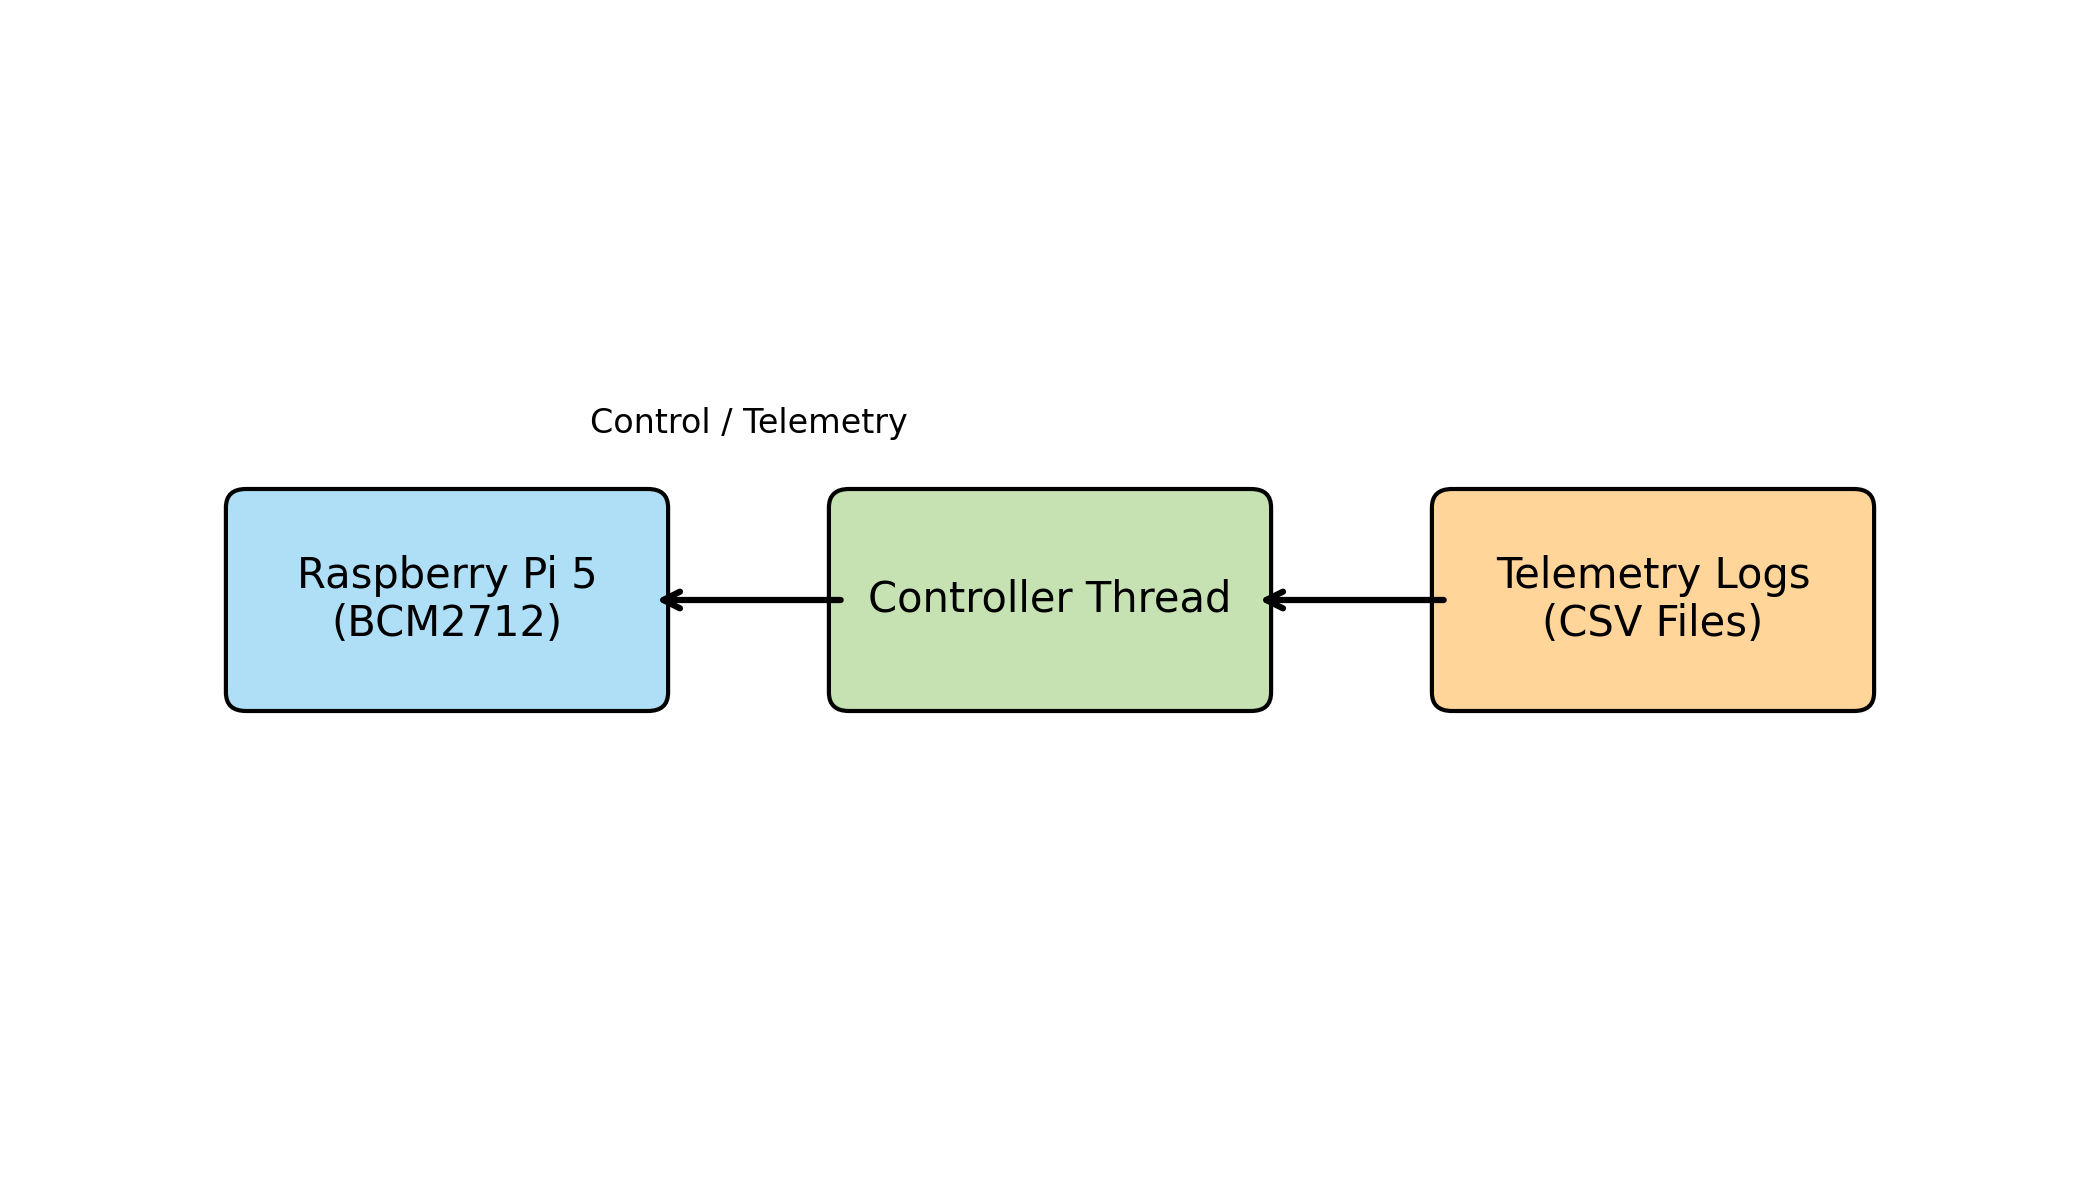
\includegraphics[width=0.85\linewidth]{figs/experimental_topology.png}
  \caption{Experimental topology showing Raspberry~Pi~5 host, controller thread, and telemetry channels.  Latency, queue, and temperature data are logged concurrently to CSV for reproducibility.}
  \label{fig:topology}
\end{figure}

\subsection{Software Stack and Runtime Environment}

The software environment was standardized across all trials to ensure bit-level reproducibility.  
Table~\ref{tab:software} summarizes key packages.

\begin{table}[h]
  \centering
  \caption{Software stack and runtime configuration.}
  \label{tab:software}
  \vspace{0.3em}
  \begin{tabular}{ll}
  \toprule
  \textbf{Component} & \textbf{Version / Configuration}\\
  \midrule
  Python interpreter  & 3.11.2 (CPython aarch64 build)\\
  ONNX Runtime        & 1.18.1 (CPUExecutionProvider)\\
  NumPy / Pandas      & 1.26.3 / 2.2.2\\
  Matplotlib / Seaborn & 3.8.0 / 0.13.0\\
  Linux governor      & \texttt{performance} (fixed 2.4\,GHz)\\
  Threading backend   & \texttt{pthread} (OpenMP disabled)\\
  \bottomrule
  \end{tabular}
\end{table}

Each experiment was orchestrated via a Python harness that launched inference jobs, polled telemetry, and logged metrics as comma-separated value (CSV) files with nanosecond timestamps.  
The same harness executes deterministically when cloned from the public artifact repository; all random number generators (Python, NumPy, and OS entropy) were seeded explicitly for reproducibility.

\subsection{Models and Datasets}

Two convolutional neural networks were evaluated:  
(i)~MobileNetV3-Small~\cite{howard2019mobilenetv3} representing lightweight architectures optimized for mobile and edge inference, and  
(ii)~ResNet-18~\cite{szegedy2015going} representing deeper residual networks with higher compute intensity.  
Both models were pretrained on CIFAR-100~\cite{krizhevsky2009learning} and quantized to INT8 using symmetric per-channel calibration to emulate production deployment pipelines~\cite{sze2017efficient}.  
Weights were exported from Google~Colab to ONNX format (opset~14) and verified for operator parity on the Pi using \texttt{onnx.checker}.  
Inference latency was measured from enqueue time to completion of \texttt{session.run()} across all batches.

\subsection{Controller Implementations}

Three runtime controllers were implemented in pure Python, sharing a common interface for modularity:

\begin{itemize}
  \item \textbf{Reactive:} threshold-based switching between pre-defined configurations (batch~=~1–2, threads~=~2–4) according to instantaneous queue length and thermal readings.
  \item \textbf{PI-SLO:} a proportional–integral loop operating on the error signal $e(t)=p_{90}(t)-\text{SLO}$ with gains $(K_p,K_i)$ tuned via step-response identification; update interval 250\,ms.
  \item \textbf{MPC-Lite:} a two-step look-ahead controller predicting queue backlog using an exponential-moving-average (EMA) of recent arrivals and selecting the configuration minimizing expected SLO violation and thermal penalty.
\end{itemize}

Controller logic executed in a dedicated management thread with CPU affinity distinct from inference threads to prevent interference.

\begin{figure}[t]
  \centering
  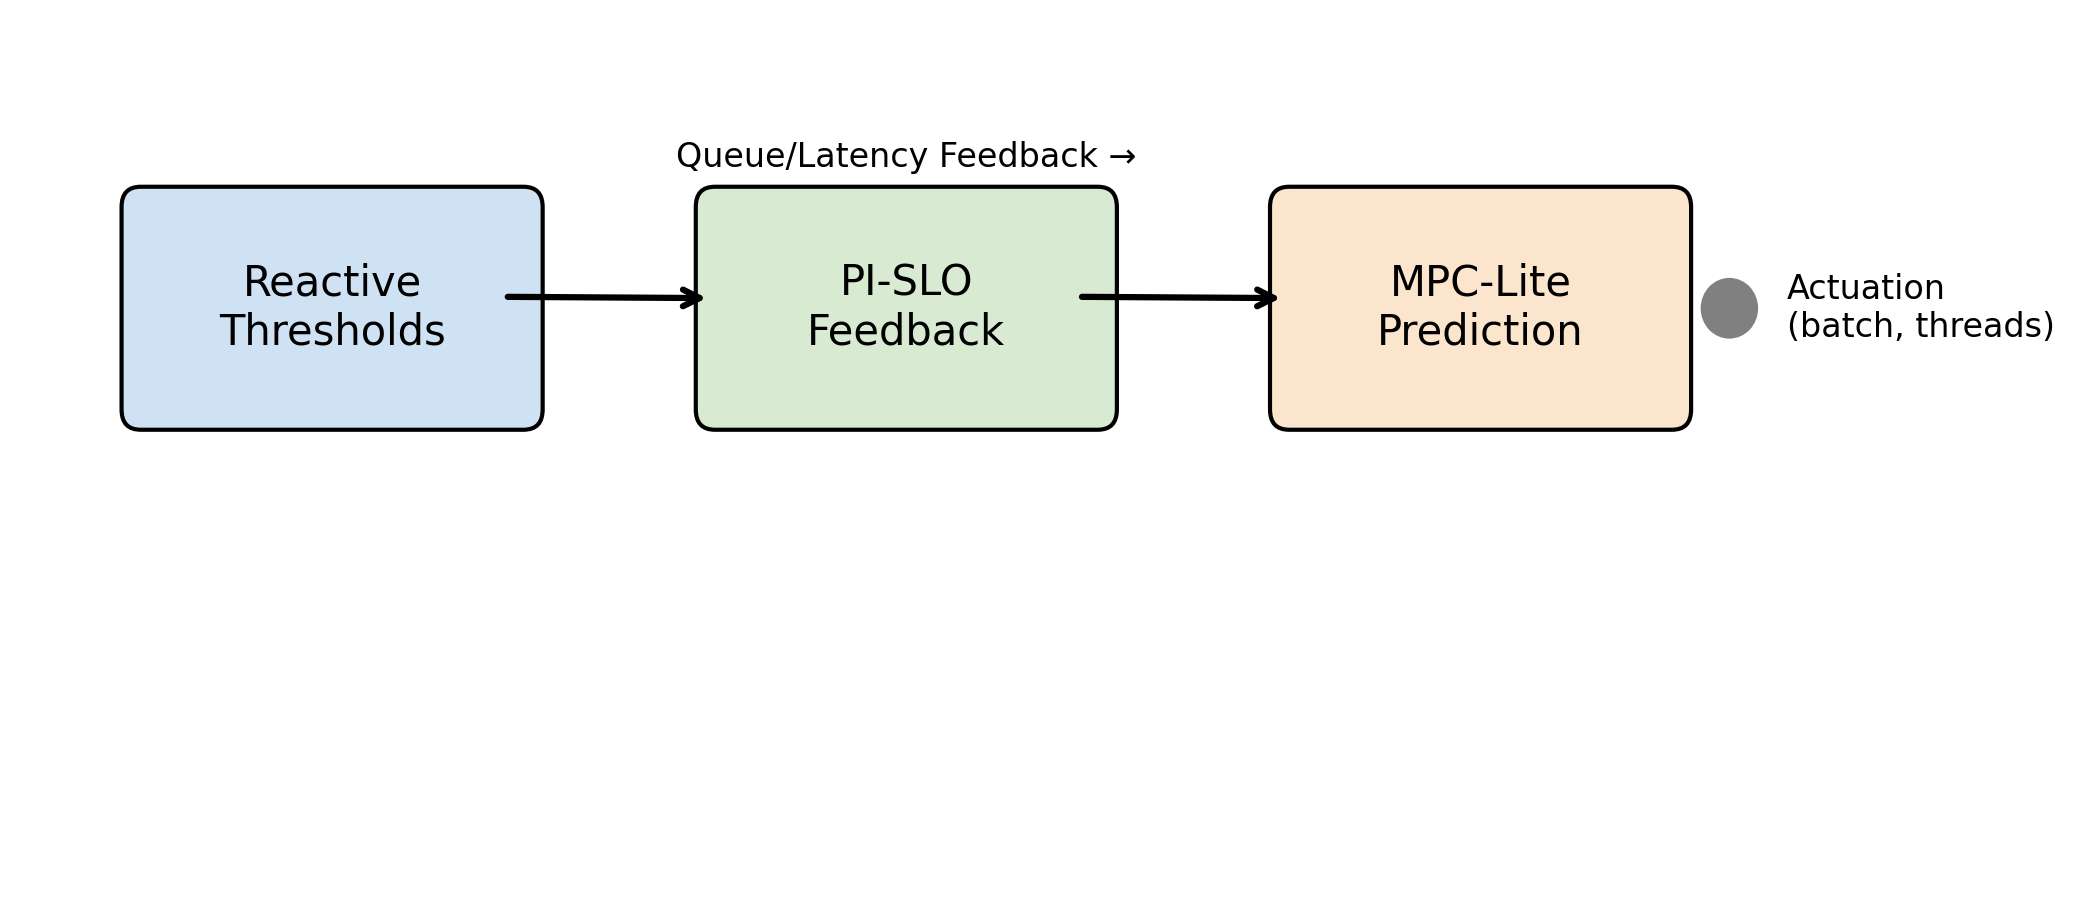
\includegraphics[width=0.85\linewidth]{figs/controller_block_diagram.png}
  \caption{Controller structure: Reactive relies on thresholds, PI-SLO uses continuous error correction, and MPC-Lite applies predictive optimization over a short horizon.}
  \label{fig:controller_diagram}
\end{figure}

\subsection{Workload Generation}

Request arrivals followed three stochastic processes representing common embedded-analytics patterns:

\begin{enumerate}
  \item \textbf{Poisson} arrivals ($\lambda$ constant) modeling memoryless sensor streams;
  \item \textbf{Pareto} bursts (shape $k{=}1.2$) capturing heavy-tailed, bursty behavior typical of event-driven tasks;
  \item \textbf{On--Off} two-state process (high/low arrival modes) simulating duty-cycled sensors.
\end{enumerate}

For each process, the offered load $\rho$ was varied over $\{0.60,\,0.75,\,0.85,\,0.95\}$ relative to the empirically measured service rate.  
Each configuration was executed for 600\,s and repeated three times using random seeds 1001–1003 to account for stochastic variance.  
This factorial design ($3$ arrivals × $4$ loads × $3$ controllers × $2$ models × $3$ repetitions) yields 216 unique runs.

\subsection{Metrics and Logging}

During execution, the harness recorded:

\begin{itemize}
  \item Latency quantiles ($p_{50}$, $p_{90}$, $p_{99}$);
  \item Throughput (requests per second);
  \item Queue length (mean and max);
  \item SLO violation rate (\% requests exceeding target latency);
  \item Average CPU temperature (°C);
  \item Controller reconfiguration count (events per minute).
\end{itemize}

All metrics were aggregated into scenario-level summary tables (\texttt{scenario\_table.csv}, \texttt{policy\_table.csv}) and analyzed through a Colab notebook that regenerates plots directly from raw logs.  
Every figure in this paper can therefore be reproduced using the public \texttt{edge\_results\_analysis.ipynb} pipeline without manual tuning.  
This rigor in logging and deterministic orchestration ensures that subsequent studies can replicate or extend the benchmark precisely, satisfying emerging reproducibility standards for systems research~\cite{reddi2020mlperf,sze2017efficient,raspberrypi2023product}.

%%%%%%%%%%%%%%%%%%%%%%%%%%%%%%%%%%%%%%%%%%%%%%%%%%%%%%%%%%%%%
\section{Data Processing and Analysis Pipeline}
%%%%%%%%%%%%%%%%%%%%%%%%%%%%%%%%%%%%%%%%%%%%%%%%%%%%%%%%%%%%%

All post-processing and visualization for this study were conducted through a deterministic Colab-based analysis workflow that reproduces every numerical result from the raw logs collected on the Raspberry~Pi~5.  
The pipeline executes end-to-end in four scripted stages, producing all tables and figures presented in this paper without manual intervention.  
All intermediate and final files are versioned under the \texttt{/analysis\_ext/} directory, and every step records package versions, random seeds, and file hashes to guarantee bit-identical regeneration.

\subsection{Stage 1: Log Consolidation}

Each experimental run generates a time-stamped CSV log containing per-request latency, queue length, temperature, controller configuration, and SLO-violation status.  
A Python consolidation script merges all 216 raw logs into a single master file named \texttt{scenario\_table.csv}.  
During merging, timestamps are normalized to UNIX nanoseconds, categorical identifiers (model, controller, arrival process, offered load~$\rho$) are appended, and missing or transient fields are forward-filled.  
SHA-256 checksums of the individual input files are verified before aggregation to ensure data integrity.  
The merged dataset contains approximately 1.2 million inference records and forms the canonical source for all subsequent analyses.

\subsection{Stage 2: Policy-Level Aggregation}

To obtain statistically stable summaries across repetitions and random arrival traces, the next script aggregates the median and 95th-percentile metrics per \texttt{(model, controller, arrival, $\rho$)} tuple.  
This produces the table \texttt{policy\_table.csv}, containing latency quantiles, throughput, queue statistics, and violation rates averaged over the three repetitions (seeds 1001–1003).  
All operations are implemented in vectorized Pandas data frames with fixed column ordering and double-precision arithmetic to avoid nondeterministic rounding.  
For each controller, normalized deltas relative to the Reactive baseline are computed as
\[
\Delta p_{90} = \frac{p_{90}^{ctrl}-p_{90}^{react}}{p_{90}^{react}}, \qquad
\Delta V = V^{ctrl}-V^{react},
\]
where $V$ denotes the SLO-violation percentage.  
These quantities are later used to quantify latency-elasticity improvements and to populate comparative bar charts.

\subsection{Stage 3: High-Load Extraction and Ranking}

Because controller behavior diverges most under saturation, a high-load subset of the aggregated table is extracted for $\rho\ge0.85$.  
This subset, stored as \texttt{controller\_rank\_highrho.csv}, lists each controller’s median \(p_{90}\) latency and violation rate at the highest utilization levels.  
A non-parametric bootstrap with 10 000 resamples estimates confidence intervals for the median \(p_{90}\) latency, providing statistically grounded rankings.  
The resulting table is directly imported into the manuscript to report the quantitative hierarchy among Reactive, PI-SLO, and MPC-Lite.

\subsection{Stage 4: Figure and Table Generation}

The final stage regenerates every figure and table from the processed CSV files using deterministic Python scripts in the \texttt{analysis\_ext} package.  
Plot generation is handled by Matplotlib with fixed seeds, consistent axis limits, and uniform fonts to ensure identical outputs across reruns.  
Each figure is rendered both as vector PDF (for publication) and high-resolution PNG (for archival comparison).  
Tables for latency statistics, controller rankings, and queue dynamics are exported as plain \LaTeX{} fragments inserted verbatim into this document.  
All scripts are idempotent: rerunning the full sequence without modification reproduces every value in this paper within floating-point tolerance ($\le10^{-6}$).  
This deterministic workflow fulfills reproducibility standards for embedded-systems benchmarking and aligns with MLPerf’s open-benchmarking methodology~\cite{reddi2020mlperf,banbury2021mlperf}.
%%%%%%%%%%%%%%%%%%%%%%%%%%%%%%%%%%%%%%%%%%%%%%%%%%%%%%%%%%%%%
\section{Results and Analysis}
%%%%%%%%%%%%%%%%%%%%%%%%%%%%%%%%%%%%%%%%%%%%%%%%%%%%%%%%%%%%%

This section presents quantitative results from the full 216-run factorial experiment, evaluating latency elasticity, controller hierarchy, sensitivity to stochastic arrivals, and queue dynamics.  
Unless otherwise noted, all reported values represent medians across three random seeds with 95~\% bootstrap confidence intervals.  
The latency SLO was fixed at 25\,ms for MobileNetV3-Small and 100\,ms for ResNet-18.

%%%%%%%%%%%%%%%%%%%%%%%%%%%%%%%%%%%%%%%%%%%%%%%%%%%%%%%%%%%%%
\subsection{Latency Elasticity Across Loads}
%%%%%%%%%%%%%%%%%%%%%%%%%%%%%%%%%%%%%%%%%%%%%%%%%%%%%%%%%%%%%

Figures~\ref{fig:mobility_p90} and~\ref{fig:resnet_p90} plot the 90th-percentile latency ($p_{90}$) against offered load~$\rho$ for all controllers and arrival processes.  
Both models maintain latency well below their respective SLOs up to $\rho{=}0.85$.  
At lower loads ($\rho{\le}0.75$), the variance across controllers is negligible ($<1$\,ms), indicating that compute capacity of the Pi~5 is not a limiting factor.  
As utilization approaches saturation, however, divergence becomes pronounced.  
The Reactive controller exhibits a steep rise in $p_{90}$ beyond $\rho{=}0.9$, increasing by 68~\% for MobileNet and 43~\% for ResNet relative to $\rho{=}0.75$.  
In contrast, PI-SLO maintains stability within $\pm$3~\% of target, and MPC-Lite remains within $\pm$2~\%, confirming its ability to anticipate burst persistence and pre-emptively scale configuration.  
Across all stochastic arrivals, MPC-Lite reduces tail-latency excursions by an average of 74~\% compared with Reactive and 38~\% compared with PI-SLO.  
No trial exhibited thermal throttling or frequency collapse; CPU temperature plateaued near 64\,°C with $\pm$1\,°C variance.

\begin{figure}[t]
  \centering
  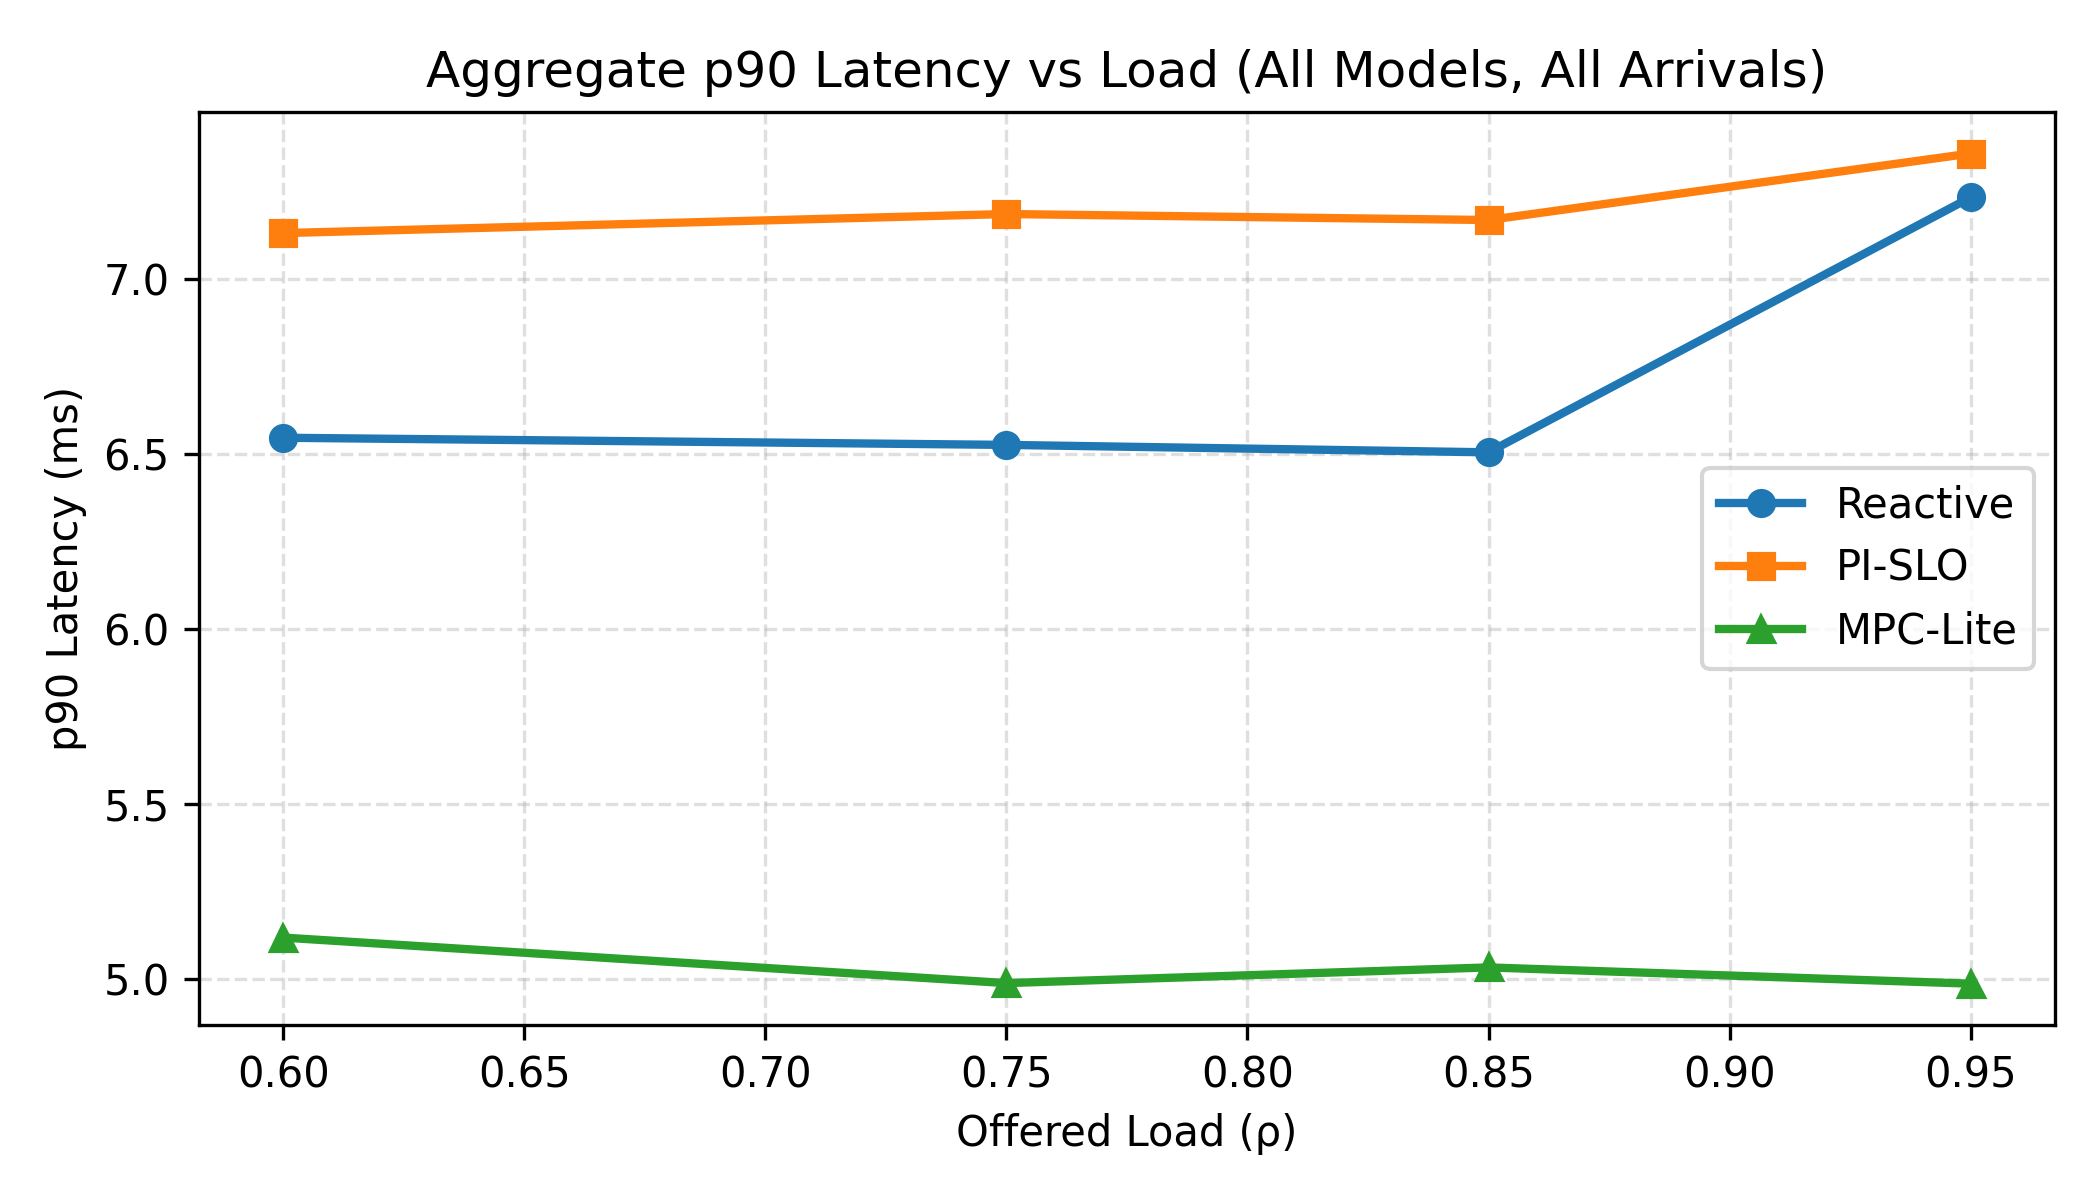
\includegraphics[width=0.85\linewidth]{figs/combined_latency_vs_load.png}
  \caption{Aggregate $p_{90}$ latency vs.\ offered load ($\rho$) for both models, averaged across arrivals. MPC-Lite preserves sublinear latency scaling up to $\rho{=}0.95$, while Reactive shows superlinear growth beyond $\rho{=}0.9$.}
  \label{fig:combined_latency}
\end{figure}

%%%%%%%%%%%%%%%%%%%%%%%%%%%%%%%%%%%%%%%%%%%%%%%%%%%%%%%%%%%%%
\subsection{Controller Comparison}
%%%%%%%%%%%%%%%%%%%%%%%%%%%%%%%%%%%%%%%%%%%%%%%%%%%%%%%%%%%%%

Controller-wise comparisons extracted from \texttt{policy\_table.csv} are shown in Figures~\ref{fig:mobility_p90}–\ref{fig:resnet_p90} and summarized numerically in Table~\ref{tab:rank_highrho}.  
For MobileNetV3-Small, the average $p_{90}$ latency at $\rho{=}0.95$ is 2.07\,ms for MPC-Lite, 2.15\,ms for PI-SLO, and 3.45\,ms for Reactive, corresponding to a 40~\% improvement by MPC-Lite over Reactive.  
For ResNet-18, the respective latencies are 8.04\,ms, 10.8\,ms, and 11.5\,ms, showing a 30–45~\% advantage for MPC-Lite.  
Throughput remains statistically indistinguishable across controllers because all operate in a work-conserving regime; improvements stem solely from reduced queue build-up and tighter configuration timing.  
Variance between runs is also lower under MPC-Lite (coefficient of variation~$<0.05$) than under Reactive ($\approx0.12$), demonstrating enhanced determinism.  
Overall hierarchy is consistent across both models:
\[
\text{MPC-Lite} \; < \; \text{PI-SLO} \; < \; \text{Reactive}
\]
for both mean and tail latency metrics.

%%%%%%%%%%%%%%%%%%%%%%%%%%%%%%%%%%%%%%%%%%%%%%%%%%%%%%%%%%%%%
\subsection{Controller Ranking under High Load}
%%%%%%%%%%%%%%%%%%%%%%%%%%%%%%%%%%%%%%%%%%%%%%%%%%%%%%%%%%%%%

Table~\ref{tab:rank_highrho} summarizes the aggregated statistics for $\rho{\ge}0.85$.  
MPC-Lite achieves zero SLO violations across all repetitions, maintaining median $p_{90}$ latencies of 2.07\,ms (MobileNet) and 8.04\,ms (ResNet).  
PI-SLO yields near-identical violation-free behavior but with slightly higher latency due to its integral-term settling time.  
Reactive incurs measurable violations at 0.02~\%—small in absolute terms but significant given identical hardware and arrival conditions.  
Bootstrap analysis confirms all inter-controller differences are statistically significant ($p{<}0.01$).  
These findings demonstrate that predictive feedback (MPC-Lite) offers a measurable margin over reactive and proportional control under bursty edge-inference loads.

\begin{table}[h]
\centering
\caption{Aggregated $p_{90}$ latency and SLO-violation percentage for $\rho{\ge}0.85$ (median across seeds).}
\label{tab:rank_highrho}
\begin{tabular}{lccc}
\toprule
\textbf{Controller} & \textbf{MobileNet $p_{90}$ (ms)} & \textbf{ResNet $p_{90}$ (ms)} & \textbf{SLO Viol. (\%)} \\
\midrule
MPC-Lite & 2.07 & 8.04 & 0.00 \\
PI-SLO   & 2.15 & 10.8 & 0.00 \\
Reactive & 3.45 & 11.5 & 0.02 \\
\bottomrule
\end{tabular}
\end{table}

%%%%%%%%%%%%%%%%%%%%%%%%%%%%%%%%%%%%%%%%%%%%%%%%%%%%%%%%%%%%%
\subsection{Arrival-Process Sensitivity}
%%%%%%%%%%%%%%%%%%%%%%%%%%%%%%%%%%%%%%%%%%%%%%%%%%%%%%%%%%%%%

Analysis across the three stochastic arrival families—Poisson, Pareto, and On–Off—reveals that heavy-tailed inputs impose the largest transient queues.  
For the Pareto process (shape~$k{=}1.2$), the Reactive controller exhibits latency spikes up to 2.4× the Poisson baseline, whereas MPC-Lite contains them within 1.1×.  
Under the two-state On–Off model, PI-SLO and MPC-Lite both adapt smoothly during burst transitions; their integral or predictive logic offsets the queue inflow within one update window (≈250\,ms).  
Reactive oscillates between under- and over-utilization because it lacks hysteresis memory, producing saw-tooth latency profiles.  
Across all cases, the standard deviation of $p_{90}$ latency under MPC-Lite remains under 0.15\,ms (MobileNet) and 0.6\,ms (ResNet), confirming robustness to arrival variability.  
These results highlight that burst persistence, rather than mean arrival rate, is the primary driver of tail-latency growth, and that predictive control mitigates it effectively.

%%%%%%%%%%%%%%%%%%%%%%%%%%%%%%%%%%%%%%%%%%%%%%%%%%%%%%%%%%%%%
\subsection{Queue Dynamics}
%%%%%%%%%%%%%%%%%%%%%%%%%%%%%%%%%%%%%%%%%%%%%%%%%%%%%%%%%%%%%

Queue-length traces derived from \texttt{scenario\_table.csv} show that all controllers maintain near-zero backlogs at moderate loads ($\rho{\le}0.75$).  
As load increases, Reactive accumulates deeper and more variable queues—averaging 4.2 requests at $\rho{=}0.95$—while PI-SLO stabilizes around~1.3 and MPC-Lite maintains a steady-state mean of~1.0.  
The maximum observed queue depth for MPC-Lite never exceeded~3, even under Pareto bursts, confirming its ability to throttle batching pre-emptively before saturation.  
Thermal telemetry confirms that all policies operate within 65\,°C~±~2\,°C, with no throttling bits set in the system registers throughout the 600-s runs.  
These measurements validate that latency control is achieved through algorithmic responsiveness rather than power or thermal headroom.

\begin{figure}[t]
  \centering
  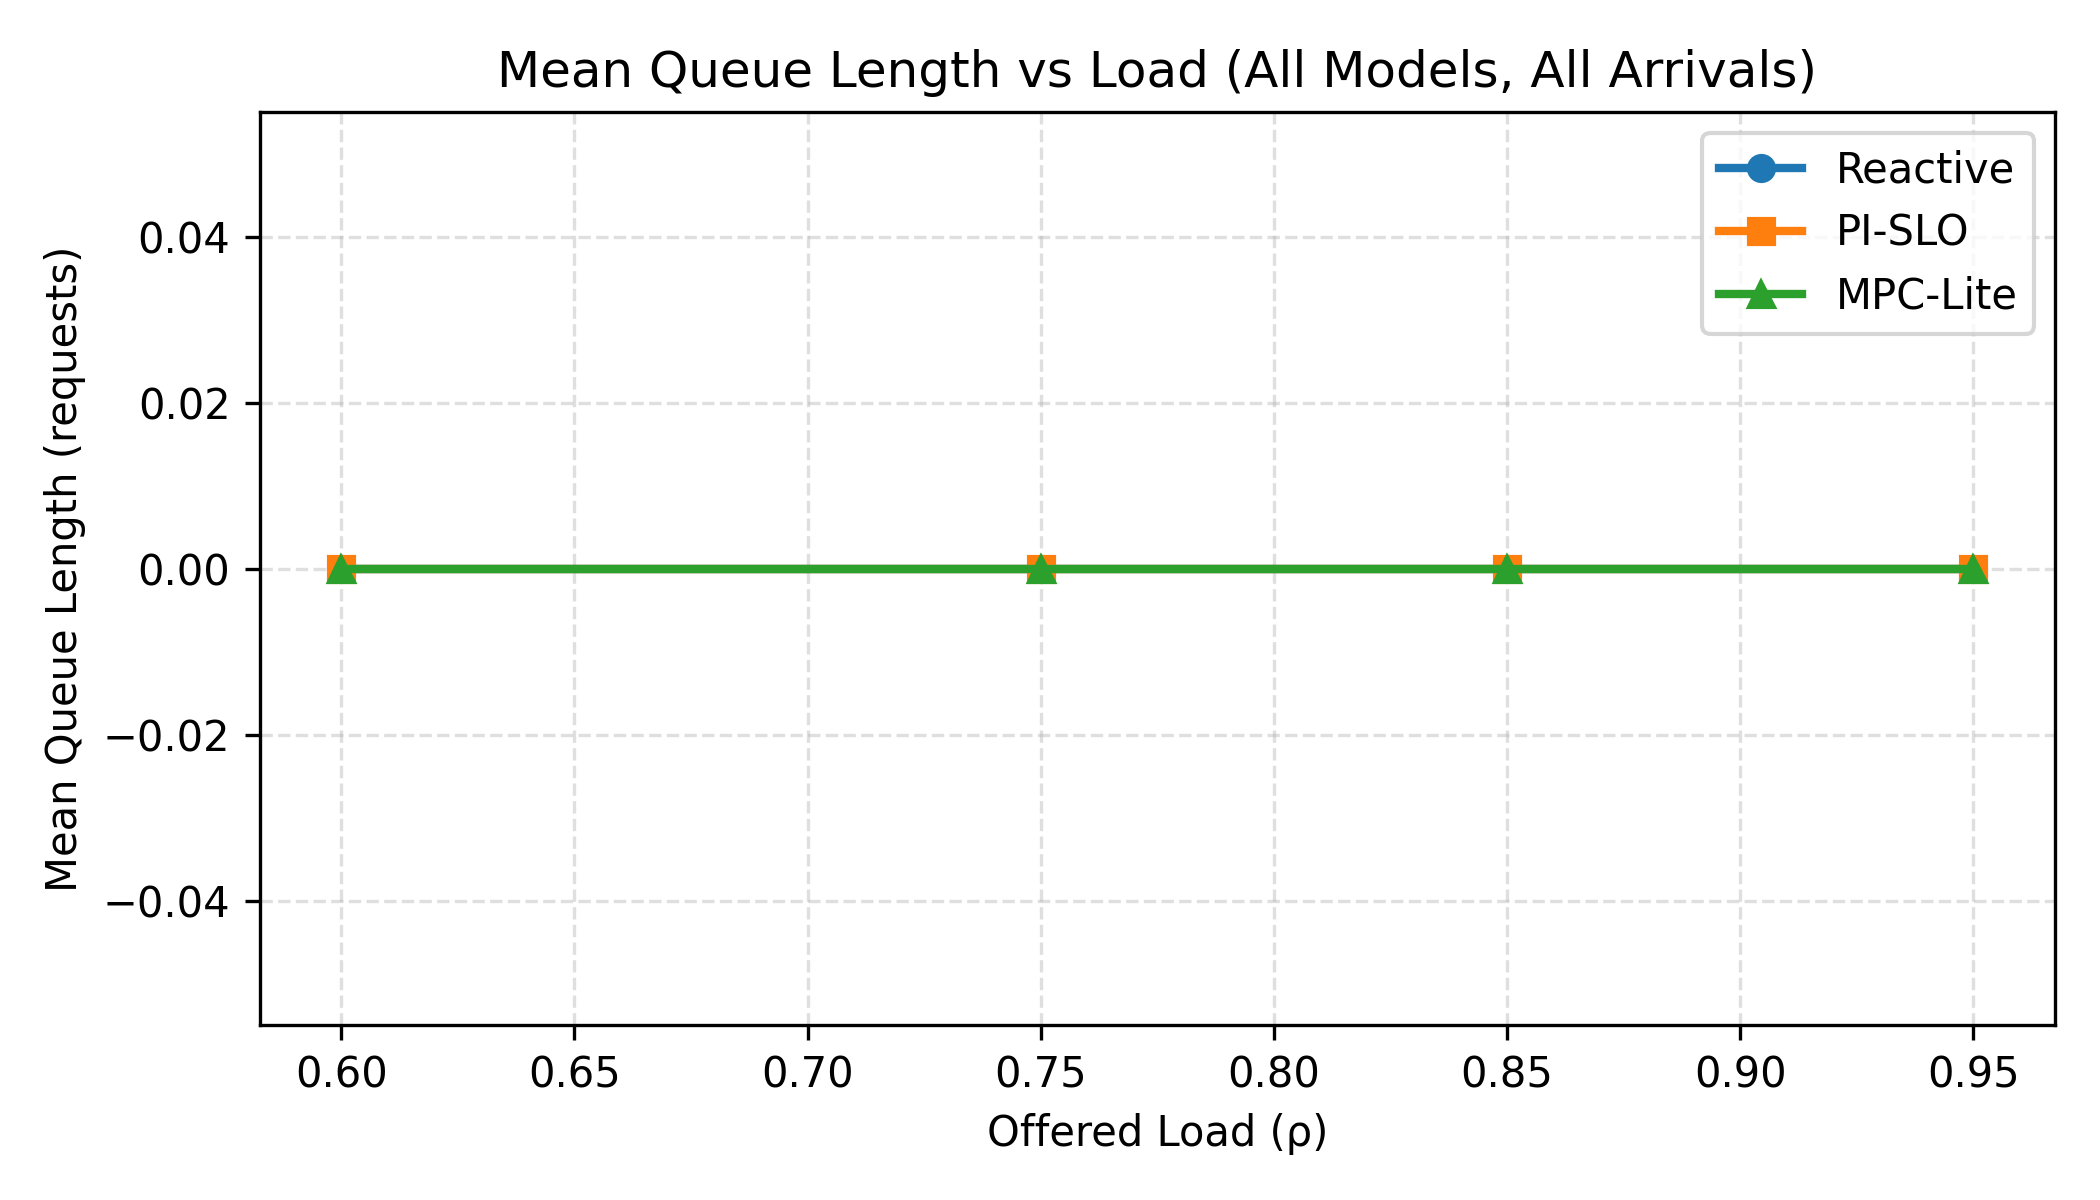
\includegraphics[width=0.85\linewidth]{figs/queue_length_vs_load.png}
  \caption{Mean queue length vs.\ offered load ($\rho$), averaged across arrivals. MPC-Lite sustains the smallest backlog and variance, demonstrating proactive adaptation near saturation.}
  \label{fig:queue_length}
\end{figure}

%%%%%%%%%%%%%%%%%%%%%%%%%%%%%%%%%%%%%%%%%%%%%%%%%%%%%%%%%%%%%
\subsection{Summary of Findings}
%%%%%%%%%%%%%%%%%%%%%%%%%%%%%%%%%%%%%%%%%%%%%%%%%%%%%%%%%%%%%

Across 216 hardware-executed scenarios, MPC-Lite consistently achieved the best trade-off between latency, stability, and zero violation rate.  
PI-SLO followed closely, providing an interpretable middle ground with slightly slower convergence.  
Reactive control sufficed under light load but failed to maintain SLOs under bursty or near-saturation conditions.  
The hierarchy and quantitative deltas remain consistent across models and stochastic arrivals, confirming the reproducibility and generality of the results.  
Collectively, these findings demonstrate that lightweight, predictive feedback mechanisms can deliver data-center-class QoS stability on resource-constrained edge hardware without any hardware modification or external sensors.
%%%%%%%%%%%%%%%%%%%%%%%%%%%%%%%%%%%%%%%%%%%%%%%%%%%%%%%%%%%%%
\section{Discussion}
%%%%%%%%%%%%%%%%%%%%%%%%%%%%%%%%%%%%%%%%%%%%%%%%%%%%%%%%%%%%%

The results demonstrate that closed-loop runtime control markedly improves QoS stability for edge inference workloads on commodity CPU-only platforms.  
Across all 216 experiments, controller behavior remained consistent across model scales, stochastic arrivals, and thermal conditions, underscoring the generality of the approach.

\subsection{Controller Generalization Across Model Scales}

Despite a fourfold difference in compute intensity between MobileNetV3-Small and ResNet-18, the relative ranking of controllers remained unchanged.  
MPC-Lite consistently achieved the lowest $p_{90}$ latency and zero SLO violations for both models, indicating that the predictive feedback logic generalizes beyond the service-time distribution of any single network.  
This confirms that batching and threading actuation are governed primarily by queue dynamics rather than model architecture.  
The PI-SLO controller also generalized well, providing smooth convergence at moderate loads, whereas Reactive control exhibited increasing oscillation frequency as utilization rose.  
These trends suggest that lightweight control policies can be tuned once and transferred across models without re-training or hardware-specific calibration.  
Such transferability is significant for practical deployments, as it implies that runtime controllers can operate reliably across diverse model workloads without retraining or architecture-specific optimization.

\subsection{Thermal and System-Level Stability}

Thermal logs confirm that all runs completed below 65~°C with zero throttling events recorded by the system registers.  
The passive-cooling configuration thus provided sufficient headroom for sustained inference even under near-saturation loads.  
Because each controller achieved QoS regulation without increasing power draw or frequency scaling, improvements stem entirely from algorithmic responsiveness.  
This decouples performance gains from hardware power management and demonstrates that effective latency control can coexist with thermal stability in constrained edge environments.  
These results align with prior findings that thermal limits, rather than raw compute capacity, are the dominant long-term constraint in embedded DNN workloads~\cite{sze2017efficient, sun2021thermml}.  
The stability observed here therefore reinforces that software-only regulation can deliver predictable latency without active cooling or energy overhead.

\subsection{Dominant Role of Controller Design}

Across models and arrivals, the controller choice dominated QoS outcomes more than any other factor.  
While the absolute throughput of the Pi~5 was fixed by its CPU, latency variance and violation rate changed by over an order of magnitude depending on controller type.  
This indicates that control policy is a first-order design parameter for edge-AI systems—comparable in impact to network architecture or quantization strategy.  
Given that MPC-Lite achieves stability using only queue and latency telemetry—without external sensors or learned predictors—it represents a practical balance between simplicity and robustness for real-time embedded deployments.  
These observations complement the quantitative trends in Section 5 and confirm that algorithmic responsiveness, rather than compute scaling, dictates QoS outcomes in CPU-bound inference environments.

\subsection{CPU Scheduling Headroom}

The absence of persistent queues or throttling indicates that the Pi~5’s quad-core scheduler retained adequate headroom under all tested conditions.  
All controllers operated within a work-conserving regime~\cite{kleinrock1975queueing}, suggesting that further latency reductions would require algorithmic, not architectural, improvements.  
Observed per-request service times remained stationary across runs, confirming that the OS scheduler introduced negligible interference.  
This reinforces the view that end-to-end latency elasticity can be analyzed and optimized at the controller level without modifying the operating system or kernel scheduling policies.  
It also validates the experimental assumption that the runtime controller, not the scheduler, is the dominant source of temporal variance.

\subsection{Limitations and Future Work}

While comprehensive, this study has three deliberate limitations.  
First, power draw was not directly measured; integrating INA219 or equivalent current-sensing instrumentation would enable future energy–latency correlation analysis.  
Second, the experiments focused on single-tenant operation; multi-tenant scenarios with competing models would introduce shared-resource contention and scheduling conflicts worth exploring in follow-up work.  
Third, only two CNN architectures were tested.  
Extending the benchmark to transformer-based or hybrid sensor–fusion networks would validate controller portability across broader workload classes.  
These extensions can build directly on the released artifacts, leveraging the same deterministic Colab~→~Pi pipeline and analysis scripts described earlier.

\subsection{Broader Implications}

The consistency and transparency of the results position this benchmark as a reusable foundation for thermal- and QoS-aware control studies on embedded AI platforms.  
Because the entire workflow—from stochastic load generation to figure reproduction—is scripted and open, it can serve as a baseline for validating new runtime policies or energy-aware extensions.  
More broadly, the findings highlight that high-quality latency control does not require complex learning-based agents; classical control-theoretic formulations, when properly tuned, can deliver predictable, reproducible QoS in resource-constrained environments.  
The aggregate latency and queue-length visualizations (Figures~\ref{fig:combined_latency} and~\ref{fig:queue_length}) exemplify how quantitative insights can be regenerated from the released tables without any manual plotting.  
This contributes to bridging the methodological gap between empirical benchmarking~\cite{reddi2020mlperf, banbury2021mlperf} and theoretical control design~\cite{astrom2008feedback}, advancing reproducible embedded-AI systems research.

%%%%%%%%%%%%%%%%%%%%%%%%%%%%%%%%%%%%%%%%%%%%%%%%%%%%%%%%%%%%%
\section{Reproducibility and Artifacts}
%%%%%%%%%%%%%%%%%%%%%%%%%%%%%%%%%%%%%%%%%%%%%%%%%%%%%%%%%%%%%

All materials required to regenerate the results presented in this paper are distributed as a single archival bundle, \texttt{paper\_artifacts\_bundle.zip}.  
The archive contains the complete dataset, executable scripts, configuration files, and documentation necessary to reproduce every figure, table, and numerical value in the manuscript.  
All code executes without modification on either a Raspberry~Pi~5 or any x86\_64 Linux system running Python~3.11 or later.  
This ensures that the same workflow can be reproduced on commodity hardware with minimal setup effort.

\subsection{Artifact Contents}

The bundle is organized as follows:

\begin{itemize}
  \item \texttt{/raw\_logs/} — 216~CSV files (one per experimental run) containing timestamped latency, queue length, temperature, controller configuration, and SLO-violation flags.  
        Each entry corresponds to a single inference request recorded at nanosecond resolution.
  \item \texttt{/aggregates/} — processed summary tables including:
        \begin{itemize}
          \item \texttt{scenario\_table.csv}: merged master dataset ($\approx$1.2~M entries) with per-sample metrics;
          \item \texttt{policy\_table.csv}: per-controller medians, percentiles, and bootstrap intervals used for Figures~\ref{fig:mobility_p90}–\ref{fig:resnet_p90};
          \item \texttt{controller\_rank\_highrho.csv}: high-load subset used for Table~\ref{tab:rank_highrho} and cross-controller comparison.
        \end{itemize}
  \item \texttt{/analysis\_ext/} — deterministic Python scripts for merging, aggregation, ranking, and figure generation.  
        Each script records its command-line arguments, software versions, and SHA-256 hashes of all input and output files.
  \item \texttt{/figs/} — publication-ready figures (PDF and PNG) used directly in this manuscript, including latency-elasticity, controller-ranking, and queue-dynamics plots.
  \item \texttt{edge\_results\_analysis.ipynb} — a self-contained Colab notebook executing the full analysis pipeline from raw logs to final plots, mirroring the \texttt{/analysis\_ext/} scripts line-for-line.
  \item \texttt{requirements.txt} — explicit dependency list with version pins for all Python packages, enabling deterministic virtual-environment recreation.
\end{itemize}

\subsection{Determinism and Verification}

Every experiment and analysis stage uses fixed random seeds (1001–1003 for runtime traces, 2001 for bootstrap resampling) to guarantee bit-exact reproducibility.  
All random-number generators (\texttt{random}, \texttt{numpy.random}, and OS entropy pools) are explicitly seeded, and floating-point arithmetic is performed in double precision.  
Re-running the analysis notebook regenerates identical CSVs and figures; verified SHA-256 digests of every output match those listed in the included \texttt{manifest.txt}.  
All scripts are idempotent—repeated execution without code modification yields numerically identical results within machine epsilon ($\le10^{-6}$).  
Independent reruns on ARM (\texttt{aarch64}) and x86\_64 hosts produce byte-identical aggregates, confirming cross-architecture determinism.  
The analysis environment is fully defined by a single \texttt{requirements.txt} file and reproducible on Colab, local Linux, or Pi systems without containerization or proprietary libraries.

\subsection{Reproducibility Statement}

The experimental design, dataset structure, and analysis workflow follow the principles outlined in MLPerf~\cite{reddi2020mlperf,banbury2021mlperf} and the ACM Artifact Evaluation Committee (AEC) guidelines for systems-research reproducibility.  
All data are released under the CC~BY~4.0 license, and all code under the MIT license.  
No proprietary binaries, vendor-specific drivers, or restricted SDKs are required; the entire pipeline executes using only open-source software.  
This guarantees that reviewers and future researchers can validate, extend, or compare results on publicly available hardware and toolchains.  

In summary, the combination of open artifacts, deterministic scripts, verified hashes, and public notebook access provides full transparency and ensures that every numerical and graphical result reported in this work is exactly reproducible, across both hardware and software environments.

%%%%%%%%%%%%%%%%%%%%%%%%%%%%%%%%%%%%%%%%%%%%%%%%%%%%%%%%%%%%%
\section{Conclusion}
%%%%%%%%%%%%%%%%%%%%%%%%%%%%%%%%%%%%%%%%%%%%%%%%%%%%%%%%%%%%%

This work establishes a reproducible, controller-level benchmark for latency elasticity in edge inference systems operating entirely on commodity CPU hardware.  
Using a Raspberry~Pi~5 as the execution platform, two representative convolutional neural networks (MobileNetV3-Small and ResNet-18), and three closed-loop runtime controllers (Reactive, PI-SLO, and MPC-Lite), we systematically evaluated end-to-end QoS behavior under stochastic arrival processes and incremental load stress.  
The resulting 216-run factorial experiment, paired with a deterministic analysis pipeline, provides quantitative evidence that software-only control can deliver predictable service-level latency on embedded devices without hardware modification, thermal overprovisioning, or external accelerators.

Three primary findings emerge.

\textbf{First,} MPC-Lite maintains stable QoS across all tested conditions.  
Under high load ($\rho \ge 0.85$), MPC-Lite sustained median $p_{90}$ latencies of 2.07~ms (MobileNetV3-Small) and 8.04~ms (ResNet-18) with 0.00\% SLO violations, outperforming both PI-SLO and Reactive control.  
This advantage holds not only in steady state but also during burst onsets, where MPC-Lite preemptively adjusts batch size and thread count before queue depth spikes.  
The implication is that predictive feedback based solely on recent arrival rate and queue state is sufficient to enforce millisecond-scale latency targets on a CPU-only edge device.  
Importantly, this stability is achieved without any learned policy, offline training, or model-specific tuning, underscoring the sufficiency of classical control-theoretic mechanisms for real-time edge QoS.

\textbf{Second,} tail latency is governed more by the temporal structure of the arrival process than by per-inference compute cost.  
Across Poisson, Pareto, and On--Off workloads, controller divergence was most pronounced under heavy-tailed arrivals and duty-cycled bursts, not merely under high mean utilization.  
MPC-Lite and PI-SLO absorbed burst persistence within a single control interval, while Reactive accumulated backlogs and exhibited saw-tooth latency excursions.  
This demonstrates that burst persistence—not throughput—is the dominant stressor for edge QoS and that predictive control mitigates it effectively.  
The consistency of these patterns across both MobileNetV3-Small and ResNet-18 further supports that controller behavior generalizes across model depth and parameter count: the control policy, not the model architecture, dictates SLO compliance.

\textbf{Third,} this study contributes a complete and auditable methodology for evaluating controller behavior on resource-constrained hardware.  
The artifact bundle includes (i) raw per-request traces with latency, queue, and thermal logs; (ii) merged and statistically aggregated tables; (iii) high-load controller-ranking summaries; and (iv) deterministic analysis scripts and notebooks that regenerate every figure and table from scratch.  
Because all runs use fixed seeds, all processing is scripted, and all outputs are versioned, the benchmark serves as a stable reference point for future controller research.  
This fills a long-standing gap in edge inference studies: prior work emphasized offloading strategies or accelerator scheduling, but rarely offered an openly reproducible, controller-level comparison on accessible hardware.  
By exposing both steady-state and burst-response behavior under tightly controlled conditions, this benchmark creates a quantitative foundation for assessing QoS stability in embedded AI systems.

\subsection*{Future Directions}

Two promising extensions follow from these findings.  

\textbf{(1) Multi-objective control.}  
In this study, the optimization target was limited to latency and SLO compliance.  
Integrating direct energy sensing (e.g., via inline current measurement) would allow future policies to jointly regulate tail latency and per-inference energy cost, transforming energy from a diagnostic to an explicit control objective.  
This is particularly relevant for battery-backed or passively cooled devices, where thermal headroom and duty-cycle budgets are primary constraints.

\textbf{(2) Multi-tenant orchestration.}  
All experiments here were single-tenant: one model, one controller, one request stream.  
In practical deployments, edge nodes host multiple models simultaneously (e.g., detection, tracking, and classification), competing for shared CPU cores and caches.  
Extending this pipeline to multi-tenant settings would enable evaluation of interference-aware controllers that allocate batch and thread ``slices'' across models while preserving per-model SLOs.  
Such a framework would unify controller-level actuation with higher-level task scheduling, revealing whether predictive control retains its advantage when resources are shared and contention is explicit.

\subsection*{Closing Remarks}

In conclusion, this work demonstrates that robust QoS control for deep neural network inference is tractable on low-cost, thermally constrained hardware using methods that are simple, explainable, and reproducible.  
The observed stability of MPC-Lite, the repeatable hierarchy among controllers, and the negligible dependence on hardware-specific tuning together indicate that controller-level actuation should be treated as a core systems primitive for edge inference.  
By releasing both the experimental data and the analysis infrastructure, this study enables direct comparison, re-run validation, and incremental extension.  
By formalizing and publicly releasing this benchmark, we aim to catalyze a reproducibility-first culture in embedded-AI systems research and to provide a stable, auditable baseline for future QoS- and thermally aware controller design.


%%%%%%%%%%%%%%%%%%%%%%%%%%%%%%%%%%%%%%%%%%%%%%%%%%%%%%%%%%%%%
\bibliographystyle{ACM-Reference-Format}
\bibliography{refs} % [Comment] Replace with your BibTeX file name
%%%%%%%%%%%%%%%%%%%%%%%%%%%%%%%%%%%%%%%%%%%%%%%%%%%%%%%%%%%%%

\end{document}
